\documentclass{article}
\usepackage[utf8]{inputenc}
\usepackage{tikz}
\usepackage{amsmath}
\usepackage{amssymb}
\usepackage[section]{placeins}

\title{Describing the Motion of a Line Segment Moving Along a Vertical Line}
\author{AJM432}
\date{January 2022}

\begin{document}

\maketitle

\section{Introduction and Definitions}
In this document we will derive the formulas responsible for the motion of a line segment moving along a vertical line. We will also attempt to explore the properties of such curves generated by the path of the line segment.
$\vspace{20 pt}$

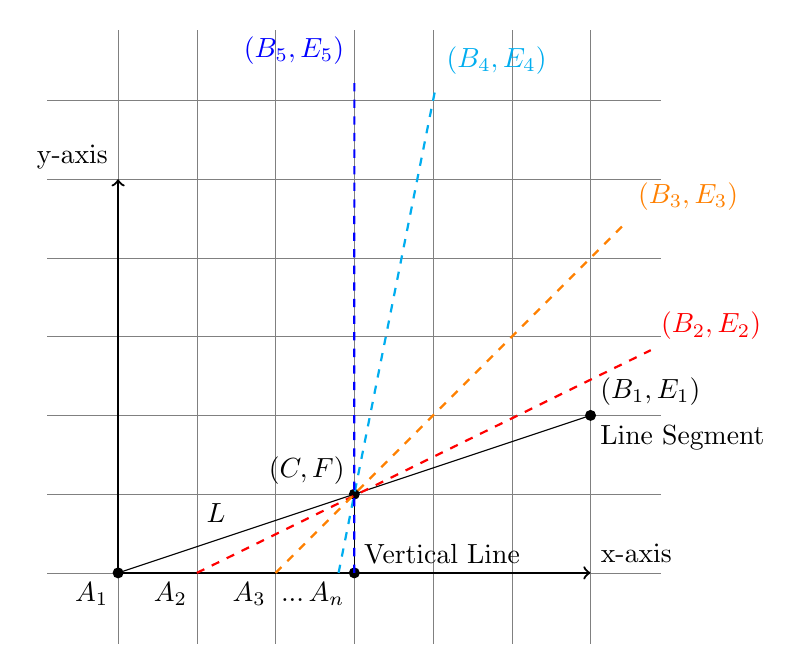
\begin{tikzpicture}

\draw[step=1cm,gray,very thin] (-0.9,-0.9) grid (6.9,6.9);
\draw[thick,->] (0,0) -- (6,0) node[anchor=south west] {x-axis};
\draw[thick,->] (0,0) -- (0,5) node[anchor=south east] {y-axis};
\draw (3, 1) node[anchor=south east] {$(C,F)$};
\draw (6, 2) node[anchor=south west] {$(B_1,E_1)$};
\draw (0, 0) node[anchor=north east] {$A_1$};
\draw (1, 0) node[anchor=north east] {$A_2$};
\draw (2, 0) node[anchor=north east] {$A_3$};
\draw (3, 0) node[anchor=north east] {$... \,A_n$};
\draw (1, 1) node[anchor=north west] {$L$};
\fill[black] (0,0) circle (0.07 cm);
\fill[black] (3,1) circle (0.07 cm);
\fill[black] (6,2) circle (0.07 cm);
\draw (3,1) -- (3,0) node[anchor=south west] {Vertical Line};
\fill[black] (3,0 ) circle (0.07 cm);
\draw (0, 0) -- (6, 2) node[anchor=north west] {Line Segment};

\draw[red, thick, dashed] (1, 0) -- (6.764523979562514, 2.8284269814872363) node[anchor=south west] {$(B_2,E_2)$};
\draw[orange, thick, dashed] (2, 0) -- (6.4721357284872845, 4.4721357284872845) node[anchor=south west] {$(B_3,E_3)$};
\draw[cyan, thick, dashed] (2.8, 0) -- (4.040347283068878, 6.201736415344387) node[anchor=south west] {$(B_4,E_4)$};
\draw[blue, thick, dashed] (2.9999, 0) -- (3.0005324554968387, 6.324554968375449) node[anchor=south east] {$(B_5,E_5)$};

\end{tikzpicture}

\vspace{1 cm}

First we will define some variables involved in the motion of the line segment.

\begin{itemize}
  \item let $L$ denote the length of the line segment
  \item let $A$ denote the distance of the tail of the line segment to the origin
  \item let $B$ denote the distance of the head of the line segment to the origin
  \item let $C$ denote the distance of the vertical line from the origin
  \item let $D$ denote the height of the tail of the line segment (since the line slides across the x-axis $D=0$ for all $A$
  \item let $E$ denote the height of the head of the line segment
  \item let $F$ denote the height of the vertical line
\end{itemize}

\section{Finding the Equation of the Line Segment}
let $g(x)=mx+h$ denote the function which describes the line segment

It follows that:

\vspace{10 pt}
$g(A) = 0$

$g(C)=F$

$g(B)=E$

\vspace{10 pt}

$$m=\frac{y_2-y_1}{x_2-x_1}$$

$$m=\frac{F}{C-A}$$

$$mA+h=0$$

$$h=-mA$$

\vspace{10 pt}


$$h=\frac{-AF}{C-A}$$

\vspace{10 pt}
$$g(x) = \frac{F}{C-A}x - \frac{AF}{C-A}$$

$$\therefore \boxed{g(x)=\frac{F(x-A)}{C-A}}$$

\section{Finding $E$ Using the Area Under the Line Segment}

Now that we have $g(x)$ we can find the area under the curve $g(x)$ in two ways\footnote{Note: we could have derived the equation for $E$ by considering the area formed by $\Delta ACF + \Delta EF(B,F) +$ the rectangle $FCB(C,F)$} since the points form $\Delta ABE$ its area is $A_{\Delta} = \frac{1}{2}E(B-A)$. We can also find the equivalent expression $\int_{A}^{B}g(x) \,dx = A_{\Delta}$. Evaluating the integral we get:

\vspace{10 pt}

$$\int_{A}^{B}g(x) \,dx = \int_{A}^{B}\frac{F(x-A)}{C-A} \,dx$$

$$=\frac{F}{C-A}\int_{A}^{B}x-A \,dx$$

$$=\frac{F}{C-A}(\frac{x^2}{2}-Ax) \Big|_{A}^{B}$$

$$\frac{1}{2}E(B-A)=\frac{F}{C-A}((\frac{B^2}{2}-AB) - (\frac{A^2}{2}-A^2))$$

$$E = \frac{2F}{(C-A)(B-A)}(\frac{1}{2}(B^2-A^2)-A(B-A))$$

$$E=\frac{2F}{(C-A)(B-A)}(\frac{1}{2}(B+A)(B-A)-A(B-A))$$

$$E=\frac{2F}{C-A}(\frac{1}{2}B-\frac{1}{2}A)$$

$$\therefore \boxed{E=\frac{F(B-A)}{C-A}}$$

\section{Finding $B$ Using the Length of the Line Segment}

The length of the line segment $L$ is the hypotenuse of the triangle with sides $(B-A)$ and $E$. Thus:

$$L^2 = (B-A)^2+E^2$$

$$L^2=(B-A)^2+\left(\frac{F(B-A)}{C-A}\right)^2$$

To simplify let $u=(B-A)$

$$L^2=u^2+\frac{u^2F^2}{(C-A)^2}$$

$$L^2 = u^2\left(1+\frac{F^2}{(C-A)^2} \right)$$

$$u^2 = \frac{L^2}{1+\left(\frac{F}{C-A}\right)^2}$$

let $v=\frac{L^2}{1+\left(\frac{F}{C-A}\right)^2}$

$$(B-A)^2=v$$

$$B^2+B(-2A)+(A^2-v)=0$$

$$B=\frac{2A \pm \sqrt{4A^2-4(A^2-v)}}{2}$$

$$B=\frac{2A \pm \sqrt{4v}}{2}$$

$A>0$ thus:
$$B=A+\sqrt{v}$$

$$B=A+\sqrt{\frac{L^2}{1+\left(\frac{F}{C-A}\right)^2}}$$

$$\therefore \boxed{B=A+ \frac{L}{\sqrt{1+\left(\frac{F}{C-A}\right)^2}}} \,\, L \geq 0$$

\section{Plotting the Parametric Curve}
Now that we have found $E$ and $B$ in terms of the defined constants we can plot them as a parametric curve since $E$ depends on $B$. We can treat ($B$,$E$) as our ($x$,$y$) components since they represent the horizontal and vertical distance of the head of the line segment respectively.

Since the line segment and the vertical line form the right $\Delta ACF$ we can assume that $C$ can be simplified into $C=\sqrt{L^2-F^2}$ as a special case for plotting the curve. Now we can plot the curve as $A \to C$ since $A$ is the only changing quantity. In the final equation we have substituted $t=A, x=B$ and $y=E$.

\[\begin{cases}
        x=t+ \frac{L}{\sqrt{1+\left(\frac{F}{C-t}\right)^2}}\\
        y=\frac{F(x-t)}{C-t}
    \end{cases}
    t\in \mathbb{R},L \geq 0, C\neq t\]

\begin{figure}[htp]
    \centering
    \includegraphics[width=10cm]{Parametric-Curve.png}
    \caption{The curve with constants $L=31$ and $F=3.5$}
    
    \vspace{1 cm}
    
    \includegraphics[width=10cm]{Curve-Small-F.png}
    \caption{The curve with constants $L=31$ and $F=0.1$}
\end{figure}

\section{Critical Point}
Notice how the curve of the above figures always reach a critical point as $A \to C$ where $B$ reaches a maxima. The critical point occurs precisely when $\dfrac{dB}{dA} = 0$ since B approaches an extrema at the critical point. Solving for the derivative of $B$ with respect to $A$ we get:

$$\dfrac{dB}{dA} = \frac{d}{dA} \left[A+ \frac{L}{\sqrt{1+\left(\frac{F}{C-A}\right)^2}}\right]$$

$$\dfrac{dB}{dA} = 1+L\frac{d}{dA}\left[\left( 1+\left(\frac{F}{C-A}\right)^2\right)^{\tfrac{-1}{2}}\right]$$

$$\dfrac{dB}{dA} = 1-\frac{L}{2}\frac{d}{dA}\left[1+\left(\frac{F}{C-A}\right)^2\right]\left(1+\left(\frac{F}{C-A}\right)^2\right)^{\tfrac{-3}{2}}$$

$$\dfrac{dB}{dA} = 1-\frac{L}{2}\left(2F^2\left(C-A\right)^{-3}\right)\left(1+\left(\frac{F}{C-A}\right)^2\right)^{\tfrac{-3}{2}}$$

$$\therefore \boxed{\dfrac{dB}{dA} = 1- \frac{LF^2}{\left(C-A\right)^3\left(1+\frac{F^2}{(C-A)^2}\right)^{\tfrac{3}{2}}}}$$

Now we can set the derivative of $B$ with respect to $A$ equal to 0 to solve for the critical point in terms of $A$.

$$\dfrac{dB}{dA} = 0$$

$$1- \frac{LF^2}{\left(C-A\right)^3\left(1+\frac{F^2}{(C-A)^2}\right)^{\tfrac{3}{2}}} = 0$$

$$(C-A)^3\left(1+\left(\frac{F}{C-A}\right)^2\right)^{\tfrac{3}{2}} = LF^2$$

let $u=C-A$

$$u^3\left(1+\frac{F^2}{u^2}\right)^{\frac{3}{2}} = LF^2$$

$$u^3\sqrt{\frac{\left(u^2+F^2\right)^3}{u^6}} = LF^2$$

$$\sqrt{\left(u^2+F^2\right)^3} = LF^2$$

$$u^2+F^2=L^{\frac{2}{3}}F^{\frac{4}{3}}$$

$$(C-A)^2 = L^{\frac{2}{3}}F^{\frac{4}{3}}-F^2$$

$$A=C - \pm \sqrt{L^{\frac{2}{3}}F^{\frac{4}{3}}-F^2}$$

$A>0$

$$\therefore \boxed{A=C - \sqrt{L^{\frac{2}{3}}F^{\frac{4}{3}}-F^2}}$$

We must evaluate $B$ at $A=C - \sqrt{L^{\frac{2}{3}}F^{\frac{4}{3}}-F^2}$ to find the x-component of the critical point which we will denote $P_x$.

$$P_x = C - \sqrt{L^{\frac{2}{3}}F^{\frac{4}{3}}-F^2}+ \frac{L}{\sqrt{1+\left(\frac{F}{C-C - \sqrt{L^{\frac{2}{3}}F^{\frac{4}{3}}-F^2}}\right)^2}}$$

$$P_x = C - \sqrt{L^{\frac{2}{3}}F^{\frac{4}{3}}-F^2}+\frac{L}{\sqrt{1+\frac{F^2}{L^{\frac{2}{3}}F^{\frac{4}{3}}-F^2}}}$$

$$\therefore \boxed{P_x = C - \sqrt{L^{\frac{2}{3}}F^{\frac{4}{3}}-F^2}+\frac{L}{\sqrt{1+\frac{1}{\left(\frac{L}{F}\right)^{\frac{2}{3}}-1}}}}$$

\vspace{1 cm}

We can now graph the vertical tangent $x=P_x$ along with our parametric equation.

\begin{figure}[htp]
    \centering
    \includegraphics[width=10cm]{curve-with-critical-point.png}
    \caption{The curve with constants $L=47$ and $F=12$}
\end{figure}

\section{Taking Limits}
As we decrease the height of the vertical line $F$, intuitively the critical point should approach $L+C$ since at the limit we are essentially sliding a line horizontally. Taking the limit as $F$ approaches 0 of $P_x$ we get:

$$\lim_{F\to0}P_x = \lim_{F\to 0}\left[C - \sqrt{L^{\frac{2}{3}}F^{\frac{4}{3}}-F^2}+\frac{L}{\sqrt{1+\frac{1}{\left(\frac{L}{F}\right)^{\frac{2}{3}}-1}}}\right]$$

$$=\lim_{F\to0}C-\lim_{F\to0}\left[\sqrt{L^{\frac{2}{3}}F^{\frac{4}{3}}-F^2}\right] + \lim_{F\to0}\left[\frac{L}{\sqrt{1+\frac{1}{\left(\frac{L}{F}\right)^{\frac{2}{3}}-1}}}\right]$$

$$=C-0+\frac{L}{\sqrt{1+\lim\limits_{F \to 0}\left[\frac{1}{\left(\frac{L}{F}\right)^{\frac{2}{3}}-1}\right]}}$$

$$=C+\frac{L}{\sqrt{1+\frac{1}{\infty}}}$$

$$\therefore \boxed{\lim_{F\to0}P_x =C+L}$$

\end{document}
